\documentclass[11pt,a4paper]{article}

% ============================================================
%  PACKAGES
% ============================================================
\usepackage[a4paper,margin=1in]{geometry}
\usepackage{graphicx}
\usepackage{xcolor}
\usepackage{tikz}
\usetikzlibrary{shapes.geometric,arrows.meta,positioning,fit,backgrounds,calc}
\usepackage{listings}
\usepackage{fancyhdr}
\usepackage{titlesec}
\usepackage{booktabs}
\usepackage{longtable}
\usepackage{array}
\usepackage{hyperref}
\usepackage{caption}
\usepackage{enumitem}
\usepackage{amsmath}
\usepackage{amssymb}
\usepackage{tcolorbox}
\usepackage{multicol}
\usepackage{setspace}
\usepackage{lastpage}

% ============================================================
%  COLOR PALETTE
% ============================================================
\definecolor{primaryblue}{HTML}{1B4F72}
\definecolor{accentteal}{HTML}{117A65}
\definecolor{softgray}{HTML}{F4F6F7}
\definecolor{codebg}{HTML}{F7F9FA}
\definecolor{codekw}{HTML}{1B4F72}
\definecolor{codestr}{HTML}{117A65}
\definecolor{codecom}{HTML}{7F8C8D}
\definecolor{borderline}{HTML}{D5D8DC}

% ============================================================
%  SECTION TITLE STYLE
% ============================================================
\titleformat{\section}
  {\normalfont\Large\bfseries\color{primaryblue}}
  {\thesection}{0.6em}{}[{\color{borderline}\titlerule[0.8pt]}]
\titleformat{\subsection}
  {\normalfont\large\bfseries\color{accentteal}}
  {\thesubsection}{0.6em}{}
\titleformat{\subsubsection}
  {\normalfont\normalsize\bfseries\color{primaryblue!80!black}}
  {\thesubsubsection}{0.6em}{}

% ============================================================
%  HEADER / FOOTER
% ============================================================
\pagestyle{fancy}
\fancyhf{}
\renewcommand{\headrulewidth}{0.6pt}
\renewcommand{\footrulewidth}{0.4pt}
\fancyhead[L]{\small\textcolor{primaryblue}{\textbf{Retainly}: Architecture, Verification \& Testing}}
\fancyhead[R]{\small\textcolor{primaryblue}{Punjab College, Burewala}}
\fancyfoot[L]{\small Ref: RBURICSPM2600539}
\fancyfoot[C]{\small\thepage\ of \pageref{LastPage}}
\fancyfoot[R]{\small Retainly Whitepaper}

% ============================================================
%  CODE LISTINGS STYLE (Dart / generic)
% ============================================================
\lstdefinelanguage{Dart}{
  keywords=[1]{class, extends, implements, final, const, var, void, return, if, else, for, while, async, await, Future, static, import, package, new, this, null, true, false, factory, enum, switch, case, break, continue, try, catch, finally, throw, is, as, get, set, required, late, extension, mixin, abstract},
  keywords=[2]{int, double, String, bool, List, Map, num, dynamic, Object},
  sensitive=true,
  morecomment=[l]{//},
  morecomment=[s]{/*}{*/},
  morestring=[b]',
  morestring=[b]"
}

\lstdefinestyle{codeStyle}{
  backgroundcolor=\color{codebg},
  basicstyle=\ttfamily\footnotesize,
  keywordstyle=[1]\color{codekw}\bfseries,
  keywordstyle=[2]\color{accentteal},
  commentstyle=\color{codecom}\itshape,
  stringstyle=\color{codestr},
  numbers=left,
  numberstyle=\tiny\color{gray},
  numbersep=8pt,
  frame=single,
  rulecolor=\color{borderline},
  framerule=0.5pt,
  breaklines=true,
  breakatwhitespace=false,
  tabsize=2,
  showstringspaces=false,
  captionpos=b,
  xleftmargin=1em,
  xrightmargin=0.5em,
  aboveskip=8pt,
  belowskip=8pt
}
\lstset{style=codeStyle, language=Dart}

% ============================================================
%  MISC
% ============================================================
\hypersetup{
  colorlinks=true,
  linkcolor=primaryblue,
  citecolor=accentteal,
  urlcolor=accentteal,
  pdftitle={Retainly: An Offline-First Adaptive Study Planner},
  pdfauthor={Muhammad Uzair},
  pdfsubject={Software Architecture and Verification Whitepaper}
}
\setlength{\parskip}{4pt}
\onehalfspacing

% ============================================================
%  TITLE PAGE
% ============================================================
\begin{document}

\begin{titlepage}
\centering
\vspace*{0.4cm}
\IfFileExists{figs/logo.png}{\includegraphics[width=2.6cm]{figs/logo.png}}{
\begin{tikzpicture}[baseline=(base.base)]
  \definecolor{appgreen}{HTML}{10B981}
  \definecolor{badgeblack}{HTML}{1F2937}
  \fill[rounded corners=12pt, appgreen] (0,0) rectangle (2.8,2.8);
  \draw[white, line width=3pt, line join=round]
    (0.7,1.85) -- (0.7,0.95)
    -- (1.05,0.75)
    arc[start angle=180, end angle=0, x radius=1.05cm, y radius=0.55cm]
    -- (2.1,0.95) -- (2.1,1.85)
    arc[start angle=0, end angle=180, x radius=1.05cm, y radius=0.55cm]
    -- cycle;
  \draw[line width=2.5pt, line cap=round, line join=round, badgeblack]
    (2.1,0.35) circle (0.38cm);
  \draw[line width=2.8pt, line cap=round, line join=round, white]
    (1.86,0.38) -- (2.02,0.54) -- (2.32,0.24);
  \coordinate (base) at (1.4,0);
\end{tikzpicture}}\\[0.6cm]

{\scshape\Large Punjab College, City Burewala\par}
\vspace{0.15cm}
{\large Department of Computer Science\par}
\vspace{1.0cm}

{\color{borderline}\rule{\linewidth}{0.8pt}}\\[0.5cm]

{\Huge\bfseries\color{primaryblue} Retainly\par}
\vspace{0.3cm}
{\Large An Offline-First, Adaptive Study Planner for Pakistani Matric Students:\par}
\vspace{0.15cm}
{\large\itshape System Architecture, Verification, and Testing Whitepaper\par}
\vspace{0.5cm}
{\color{borderline}\rule{0.6\linewidth}{0.5pt}}\\[0.8cm]

\begin{tabular}{rl}
\textbf{Author:} & Muhammad Uzair \\[4pt]
\textbf{Institute:} & Punjab College, City Burewala \\[4pt]
\textbf{Reference No.:} & RBURICSPM2600539 \\[4pt]
\textbf{Project:} & Retainly --- Offline Study Planner (Flutter) \\[4pt]
\textbf{Date:} & \today \\[4pt]
\end{tabular}

\vfill

{\small\itshape ``All core study data stays on-device by default; online features are optional and consent-gated.''\par}
\vspace{0.5cm}
{\small Prepared as a technical whitepaper accompanying the Retainly competition submission.\par}

\end{titlepage}

% ============================================================
%  ACKNOWLEDGMENT
% ============================================================
\section*{Acknowledgment}
\addcontentsline{toc}{section}{Acknowledgment}
\begin{tcolorbox}[colback=softgray,colframe=borderline,boxrule=0.6pt,arc=2pt,left=10pt,right=10pt,top=8pt,bottom=8pt]
This whitepaper was prepared with the assistance of an AI writing and analysis tool (Claude, by Anthropic), which was used to analyze the codebase structure, help draft explanatory text, and typeset this document. All source code discussed herein, all engineering decisions, and the correctness, integrity, and originality of the underlying \textbf{Retainly} application remain the sole responsibility of the author, \textbf{Muhammad Uzair}. The AI tool was used strictly as a writing and documentation aid and did not author the software itself; all code was written, reviewed, and is owned by the author.
\end{tcolorbox}

\vspace{0.4cm}

% ============================================================
%  ABSTRACT
% ============================================================
\section*{Abstract}
\addcontentsline{toc}{section}{Abstract}
Retainly is an offline-first Flutter application that converts a Matric (Class 9--10) syllabus into an adaptive daily study plan, tracks focused study sessions, and drives spaced-repetition revision, with optional AI assistance and encrypted local backups. This whitepaper documents the system's layered architecture, its core algorithms --- a priority-weighted daily task scheduler and an SM-2 spaced-repetition engine --- its consent-gated online features, and its local-first security model. It further presents the project's testing methodology, a walkthrough of concrete defects discovered and fixed during development (a synchronization data-loss bug, brute-force authentication exposure, and unencrypted backups), and the verification strategy used to gain confidence in the codebase (20{,}490 lines of Dart across a feature-first module layout, exercised by 15 unit-test suites totaling over 2{,}000 lines of test code). The paper is intended for code auditors, examiners, and future contributors who need a concise but rigorous account of how the system is built, how it fails safely, and how it has been tested.

\vspace{0.3cm}
\noindent\textbf{Keywords:} offline-first architecture, Flutter, spaced repetition (SM-2), adaptive scheduling, software verification, encrypted local backup, mobile application testing.

\newpage
\tableofcontents
\newpage

% ============================================================
%  1. INTRODUCTION
% ============================================================
\section{Introduction}

\subsection{Motivation}
Matric-level students in Pakistan preparing for board examinations typically juggle multiple subjects, an approaching exam date, uneven confidence across chapters, and inconsistent access to the internet. Existing study-planner applications are frequently cloud-dependent, ad-supported, or built around generic curricula that do not map onto the FBISE/Punjab-board syllabus structure. \textbf{Retainly} was designed to address this gap directly: it is \emph{offline-first} (all core data is stored on-device), \emph{no-account} (no login is required to use the core planner), and \emph{no-ads}, while still offering optional AI-assisted study aids and encrypted backups for users who choose to enable them.

\subsection{Goals of this Document}
This whitepaper is not a user manual; it is a technical account of the system aimed at an academic/examination audience. It aims to:
\begin{itemize}[nosep]
    \item Describe the layered software architecture and the rationale behind it.
    \item Explain the two central algorithms that drive the product experience --- the daily task scheduler and the SM-2 spaced-repetition engine --- with source excerpts.
    \item Document the security and privacy posture of the local-first data model.
    \item Present the testing strategy, coverage, and a record of problems discovered and resolved, framed as engineering case studies.
    \item Provide diagrams that make the control flow and data flow auditable without reading the full 20{,}000+ line codebase.
\end{itemize}

\subsection{System Snapshot}
\begin{table}[h!]
\centering
\begin{tabular}{ll}
\toprule
\textbf{Attribute} & \textbf{Value} \\
\midrule
Framework & Flutter (Dart SDK $\geq$ 3.7.0) \\
State management & Riverpod \\
Local storage & sqflite (mobile), Drift/FFI (desktop) \\
Navigation & GoRouter (shell + modal routes) \\
Source lines of code & 20{,}490 (lib/ + test/) \\
Feature modules & 15 (\texttt{lib/features/*}) \\
Unit test suites & 15 files, 2{,}011 lines \\
Target platforms & Android (primary), Linux desktop \\
Localization & English (Urdu RTL framework in place; full translation pending) \\
\bottomrule
\end{tabular}
\caption{High-level project statistics.}
\end{table}

% ============================================================
%  2. SYSTEM ARCHITECTURE
% ============================================================
\section{System Architecture}

\subsection{Layered Design}
Retainly follows a feature-first, layered architecture with a strict single-source-of-truth policy: the local SQLite database is authoritative for all study data, and \texttt{DatabaseRepository} is the sole intermediary between the UI and storage. Figure~\ref{fig:architecture} shows the four architectural layers and how a user action or an optional network call moves through them.

\begin{figure}[h!]
\centering
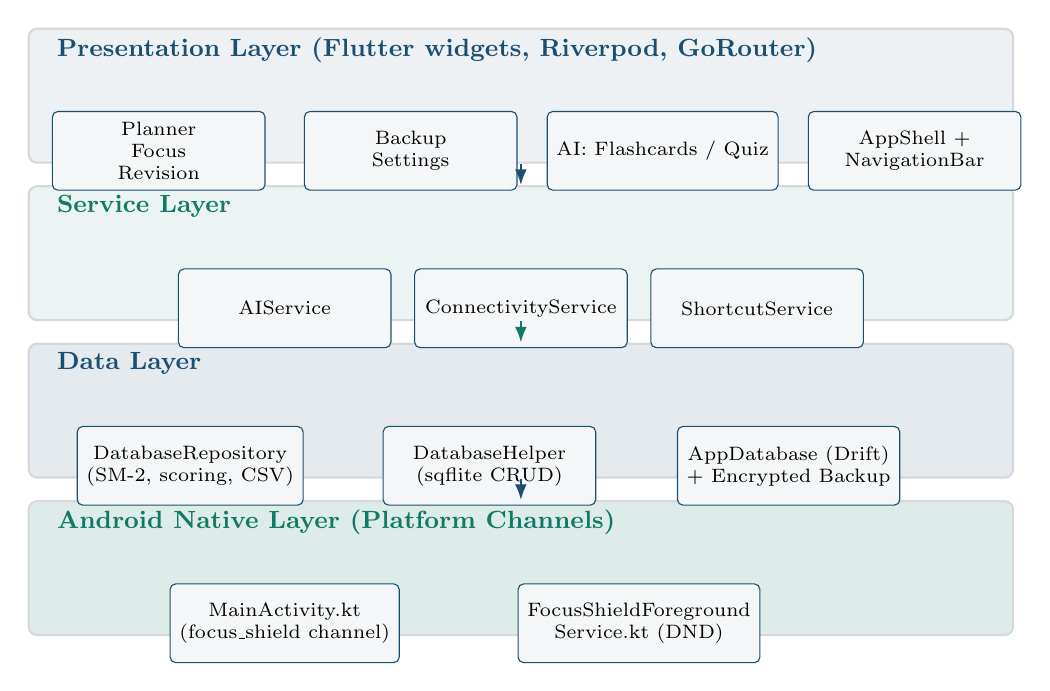
\begin{tikzpicture}[
    layer/.style={rectangle, rounded corners=3pt, draw=borderline, thick, minimum width=12.5cm, minimum height=1.7cm, align=center, font=\small},
    box/.style={rectangle, rounded corners=2pt, draw=primaryblue, fill=softgray, minimum width=2.7cm, minimum height=1cm, align=center, font=\scriptsize},
    every node/.style={font=\small}
]
% Layer bands
\node[layer, fill=primaryblue!8] (pres) at (0,6.0) {};
\node[layer, fill=accentteal!8]  (svc)  at (0,4.0) {};
\node[layer, fill=primaryblue!12] (data) at (0,2.0) {};
\node[layer, fill=accentteal!14] (native) at (0,0.0) {};

\node[anchor=north west, font=\bfseries\small\color{primaryblue}] at (pres.north west) {\ \ Presentation Layer (Flutter widgets, Riverpod, GoRouter)};
\node[anchor=north west, font=\bfseries\small\color{accentteal}] at (svc.north west) {\ \ Service Layer};
\node[anchor=north west, font=\bfseries\small\color{primaryblue}] at (data.north west) {\ \ Data Layer};
\node[anchor=north west, font=\bfseries\small\color{accentteal}] at (native.north west) {\ \ Android Native Layer (Platform Channels)};

\node[box] at (-4.6,5.3) {Planner\\Focus\\Revision};
\node[box] at (-1.4,5.3) {Backup\\Settings};
\node[box] at (1.8,5.3) {AI: Flashcards / Quiz};
\node[box] at (5.0,5.3) {AppShell +\\NavigationBar};

\node[box] at (-3.0,3.3) {AIService};
\node[box] at (0.0,3.3) {ConnectivityService};
\node[box] at (3.0,3.3) {ShortcutService};

\node[box] at (-4.2,1.3) {DatabaseRepository\\(SM-2, scoring, CSV)};
\node[box] at (-0.4,1.3) {DatabaseHelper\\(sqflite CRUD)};
\node[box] at (3.4,1.3) {AppDatabase (Drift)\\ + Encrypted Backup};

\node[box] at (-3.0,-0.7) {MainActivity.kt\\(focus\_shield channel)};
\node[box] at (1.5,-0.7) {FocusShieldForeground\\Service.kt (DND)};

\draw[-{Latex[length=2mm]}, thick, primaryblue] (pres.south) -- (svc.north);
\draw[-{Latex[length=2mm]}, thick, accentteal] (svc.south) -- (data.north);
\draw[-{Latex[length=2mm]}, thick, primaryblue] (data.south) -- (native.north);
\end{tikzpicture}
\caption{Layered architecture of Retainly: presentation calls services and the data-access facade; the data layer wraps sqflite/Drift; the Android native layer is reached only from the Focus feature via a platform channel.}
\label{fig:architecture}
\end{figure}

\subsection{Design Principles}
\begin{enumerate}[nosep]
    \item \textbf{Offline-first with graceful degradation.} Core study data (subjects, chapters, tasks, focus sessions, revision items, resources, practical records) lives in local SQLite. If network access fails --- missing configuration, no connectivity, or an unsupported platform --- the app falls back to local-only mode and all core functionality remains usable.
    \item \textbf{Single source of truth.} \texttt{DatabaseRepository} (\texttt{lib/data/repositories/database\_repository.dart}) is the only intermediary between the UI and the database; every mutation flows through it.
    \item \textbf{Domain-driven modular layout.} Non-trivial feature modules (e.g. \texttt{backup}) follow a \texttt{domain / data / presentation} split: immutable domain models, abstract repository interfaces, concrete local implementations, and a coordination layer (\texttt{BackupManager}) that composes them --- allowing interfaces to be mocked in tests without touching UI code.
    \item \textbf{Consent-gated online features.} AI assistance is opt-in, quota-limited, and only ever invoked with explicit user consent recorded locally.
\end{enumerate}

\subsection{Project Layout}
\begin{lstlisting}[language=, basicstyle=\ttfamily\scriptsize, frame=single, backgroundcolor=\color{codebg}, caption={Top-level source layout (abridged).}]
lib/
  core/        # theme, constants, feature flags, utilities
  data/        # DatabaseHelper (sqflite), Drift schema, models, repository
  services/    # AIService, ConnectivityService, ShortcutService
  providers/   # Riverpod providers (DI + state)
  navigation/  # GoRouter routes + AppShell
  features/    # planner, focus, revision, backup, ai, settings, legal, ...
  l10n/        # ARB bundles: English (Urdu RTL framework in place; full translation pending)
test/unit/     # 15 unit-test suites (services, repository, models, security)
test/widget_test.dart
android/app/src/main/kotlin/com/codesym/retainly/
  MainActivity.kt                    # focus_shield platform channel
  FocusShieldForegroundService.kt    # DND + foreground timer
\end{lstlisting}

% ============================================================
%  3. CORE ALGORITHMS
% ============================================================
\section{Core Algorithms}

\subsection{Adaptive Daily Scheduling}
The planner selects tasks that fit within the user's daily study-minute budget. Each pending task is scored by \texttt{computeTaskScore()}, which combines due-date urgency, explicit priority, and a budget-fit bonus, and the resulting list is filled greedily (a knapsack-style fill) until the daily budget is exhausted; overflow tasks are surfaced for manual rescheduling.

\begin{lstlisting}[caption={Task urgency scoring --- \texttt{lib/data/repositories/database\_repository.dart}}, label={lst:score}]
int computeTaskScore(TaskModel task, int dailyMinutes) {
  final now = DateTime.now();
  var score = 0;
  if (task.dueAt != null) {
    final diff = DateTime.parse(task.dueAt!).difference(now).inDays;
    score += diff < 0 ? 50 : (30 - diff.clamp(0, 30));
  }
  score += task.priority * 10;
  if (task.estimatedMinutes <= dailyMinutes) score += 5;
  return score;
}
\end{lstlisting}

Overdue tasks receive a flat urgency bonus of 50; tasks due within the next 30 days receive a linearly decaying bonus, so a task due tomorrow outranks one due in three weeks. Priority dominates the score (weight $\times 10$), and a small tie-breaking bonus rewards tasks that comfortably fit the remaining daily budget --- favoring plans that are actually completable over plans that merely look optimal on paper.

\subsection{Spaced Repetition (SM-2)}
Revision items use the classical SuperMemo-2 (SM-2) algorithm. A user's 0--100 confidence rating on a revision card is mapped to a 0--5 quality score; the ease factor and the next review interval are then recomputed.

\begin{lstlisting}[caption={SM-2 ease-factor and interval update --- \texttt{database\_repository.dart}}, label={lst:sm2}]
final double _sm2MinEaseFactor = 1.3;

double _sm2NewEaseFactor(double currentEaseFactor, int quality) {
  final q = quality.clamp(0, 5);
  final adjustment = 0.1 - (5 - q) * (0.08 + (5 - q) * 0.02);
  return max(_sm2MinEaseFactor, currentEaseFactor + adjustment);
}

int _sm2NewInterval(int repetitions, double easeFactor, int currentInterval) {
  if (repetitions == 0) return 1;
  if (repetitions == 1) return 6;
  if (repetitions == 2) return 15;
  return (currentInterval * easeFactor).round().clamp(1, 365);
}
\end{lstlisting}

The ease factor is bounded below at 1.3 (per the original SM-2 specification) so that a difficult item never converges to a review interval of zero. The repetition counter resets to 0 whenever quality drops below 3 (i.e., the user reports low recall confidence), which restarts the 1$\rightarrow$6$\rightarrow$15-day ramp described in the product documentation, after which the interval grows multiplicatively with the ease factor, capped at 365 days.

\begin{equation}
\text{interval}_{n} =
\begin{cases}
1 & n = 0\\
6 & n = 1\\
15 & n = 2\\
\mathrm{clamp}\!\left(\mathrm{round}(\text{interval}_{n-1}\cdot EF),\,1,\,365\right) & n \geq 3
\end{cases}
\end{equation}

% ============================================================
%  4. STATE MACHINES
% ============================================================
\section{State Machines}

\subsection{Onboarding Gate}
Navigation (\texttt{lib/navigation/app\_router.dart}) implements a two-stage redirect gate driven by two Riverpod providers: database readiness and profile existence. Figure~\ref{fig:onboarding} shows the resulting state machine.

\begin{figure}[h!]
\centering
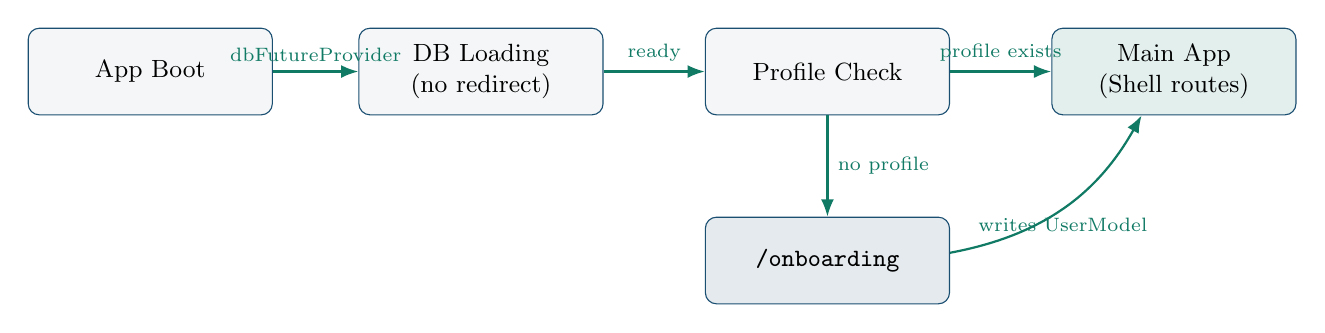
\begin{tikzpicture}[
  state/.style={rectangle, rounded corners=4pt, draw=primaryblue, fill=softgray, minimum width=3.1cm, minimum height=1.1cm, align=center, font=\small},
  every edge/.style={draw=accentteal, thick, -{Latex[length=2.2mm]}}
]
\node[state] (boot) at (0,0) {App Boot};
\node[state] (dbload) at (4.2,0) {DB Loading\\(no redirect)};
\node[state] (checkprofile) at (8.6,0) {Profile Check};
\node[state, fill=primaryblue!12] (onboard) at (8.6,-2.4) {\texttt{/onboarding}};
\node[state, fill=accentteal!12] (main) at (13.0,0) {Main App\\(Shell routes)};

\draw[-{Latex[length=2.2mm]}, thick, accentteal] (boot) -- node[above,font=\scriptsize]{dbFutureProvider} (dbload);
\draw[-{Latex[length=2.2mm]}, thick, accentteal] (dbload) -- node[above,font=\scriptsize]{ready} (checkprofile);
\draw[-{Latex[length=2.2mm]}, thick, accentteal] (checkprofile) -- node[right,font=\scriptsize]{no profile} (onboard);
\draw[-{Latex[length=2.2mm]}, thick, accentteal] (checkprofile) -- node[above,font=\scriptsize]{profile exists} (main);
\draw[-{Latex[length=2.2mm]}, thick, accentteal] (onboard) to[bend right=25] node[below,font=\scriptsize]{writes UserModel} (main);
\end{tikzpicture}
\caption{Onboarding redirect state machine implemented by \texttt{\_RouterRefreshNotifier}, listening to \texttt{dbFutureProvider} and \texttt{userProfileProvider}.}
\label{fig:onboarding}
\end{figure}

\subsection{Focus-Session Lifecycle}
The Pomodoro-style Focus feature is a three-state machine (\emph{idle} $\rightarrow$ \emph{running} $\rightarrow$ \emph{completed}), coordinated with a native Android \texttt{focus\_shield} platform channel that toggles Do-Not-Disturb via \texttt{NotificationManager.setInterruptionFilter()}, guarded by a foreground service so the OS does not reclaim the session.

\begin{figure}[h!]
\centering
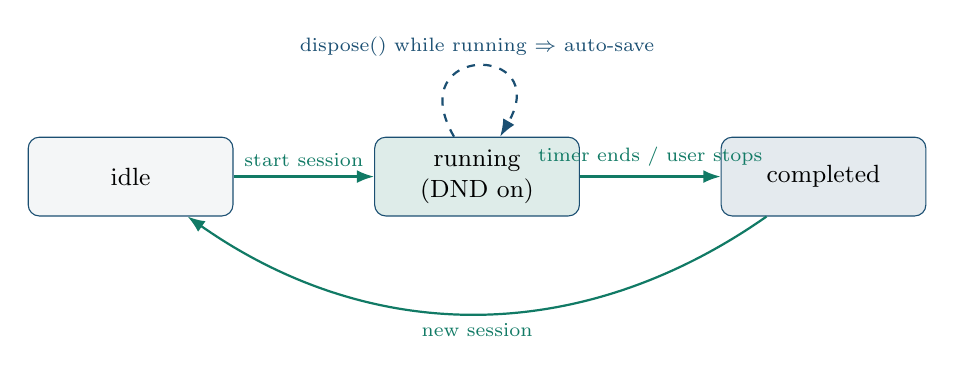
\begin{tikzpicture}[
  state/.style={rectangle, rounded corners=4pt, draw=primaryblue, fill=softgray, minimum width=2.6cm, minimum height=1cm, align=center, font=\small},
  every edge/.style={draw=accentteal, thick, -{Latex[length=2.2mm]}}
]
\node[state] (idle) at (0,0) {idle};
\node[state, fill=accentteal!14] (running) at (4.4,0) {running\\(DND on)};
\node[state, fill=primaryblue!12] (completed) at (8.8,0) {completed};

\draw[-{Latex[length=2.2mm]}, thick, accentteal] (idle) -- node[above,font=\scriptsize]{start session} (running);
\draw[-{Latex[length=2.2mm]}, thick, accentteal] (running) -- node[above,font=\scriptsize]{timer ends / user stops} (completed);
\draw[-{Latex[length=2.2mm]}, thick, accentteal] (completed) to[bend left=35] node[below,font=\scriptsize]{new session} (idle);
\draw[-{Latex[length=2.2mm]}, thick, dashed, primaryblue] (running) to[out=120,in=60,looseness=6] node[above,font=\scriptsize]{dispose() while running $\Rightarrow$ auto-save} (running);
\end{tikzpicture}
\caption{Focus-session state machine. On widget disposal mid-session, \texttt{\_saveSession()} persists progress to prevent data loss on app exit.}
\label{fig:focus}
\end{figure}

% ============================================================
%  5. SECURITY & PRIVACY
% ============================================================
\section{Security, Privacy \& Consent Model}

\subsection{Encrypted Local Backup}
Backups serialize all study entities and relevant \texttt{SharedPreferences} keys to a single JSON document, which is then encrypted with AES-256 (via the \texttt{encrypt} package) before being written to disk. The encryption key is a 32-byte securely-random key stored in \texttt{FlutterSecureStorage} (Android Keystore) where available, falling back to \texttt{SharedPreferences} on desktop targets that lack a hardware-backed keystore.

\begin{lstlisting}[caption={Backup file format marker --- \texttt{backup\_encryption\_service.dart}}]
static const _magicHeader = 'MSP_BACKUP_V1';
// file layout: [ magicHeader | 16-byte IV | AES-256-CBC ciphertext ]
\end{lstlisting}

Restore is defensive by construction: \texttt{LocalRestoreService.restoreFromFile()} validates, in order, file existence, non-empty content, successful decryption, valid JSON, presence of required fields, and schema-version compatibility, returning a structured \texttt{RestoreResult} (rather than throwing) for every failure mode so the UI can present a clear message instead of crashing.

\subsection{Consent-Gated AI}
All AI-assisted features (task breakdown, flashcards, quizzes) are gated behind four independent checks, evaluated in order, so that the most user-relevant failure reason is surfaced first:

\begin{lstlisting}[caption={AI request gating --- \texttt{lib/services/ai\_service.dart}}]
static const int _dailyQuota = 10;

Future<String?> _checkQuotaAndGate(String userId) async {
  await _resetQuotaIfNewDay();
  if (!await hasAiConsent())            return 'AI assistance requires consent in Settings.';
  if (!await hasAcceptedCostWarning())   return 'Accept the AI cost warning before using this feature.';
  if (!await hasAcceptedAiPolicy())      return 'Please accept the AI policy before using this feature.';
  final remaining = await getAiUsageQuota(userId);
  if (remaining <= 0)                    return 'Daily AI quota reached. Try again tomorrow.';
  if (!await _connectivity.isOnline)     return 'No internet connection. Connect to use AI features.';
  return null; // all gates passed
}
\end{lstlisting}

A quota of 10 requests/day/user is tracked client-side in \texttt{SharedPreferences} with date-rollover reset, and every gate returns a descriptive string rather than throwing, so a missing prerequisite degrades gracefully into a user-facing message instead of a crash.

\subsection{Security Posture Summary}
\begin{table}[h!]
\centering
\small
\begin{tabular}{p{4.4cm}p{9cm}}
\toprule
\textbf{Area} & \textbf{Posture} \\
\midrule
Local database & Plain SQLite (not OS-level encrypted); acceptable given the offline, single-user threat model, flagged as a future hardening item. \\
Backups & AES-256 encrypted, off by default, user-controlled, never auto-uploaded. \\
AI features & Opt-in consent, cost-warning acknowledgment, explicit policy acceptance, 10/day quota, connectivity gate. \\
Secrets & Encryption keys held in platform Keystore (Android) / secure fallback (desktop); never embedded in source. \\
Error surfaces & Optional features fail silently by design so a missing permission or offline network never crashes the core planner. \\
\bottomrule
\end{tabular}
\caption{Summary of the current security and privacy posture.}
\end{table}

% ============================================================
%  6. TESTING & PROBLEM SOLVING
% ============================================================
\section{Testing Methodology and Problem Solving}

\subsection{Testing Strategy}
Retainly's test suite is unit-focused, targeting the layers most likely to contain business-logic regressions: data models, the SM-2/scoring logic inside \texttt{DatabaseRepository}, the AI service's gating and retry behavior, and the backup/restore pipeline. Table~\ref{tab:tests} summarizes the 15 unit-test files (2{,}011 lines total) plus a widget smoke test.

\begin{table}[h!]
\centering
\small
\begin{tabular}{p{5.6cm}rp{6cm}}
\toprule
\textbf{Test file} & \textbf{Lines} & \textbf{Focus} \\
\midrule
\texttt{ai\_service\_test.dart} & 321 & Consent, quota, provider selection, response parsing \\
\texttt{backup\_restore\_test.dart} & 225 & Multi-layer restore failure modes \\
\texttt{backup\_manager\_screen\_test.dart} & 185 & Backup UI + manager coordination \\
\texttt{legal\_screen\_test.dart} & 165 & Legal document rendering \\
\texttt{ai\_service\_retry\_test.dart} & 163 & Exponential backoff / retry on transient failure \\
\texttt{settings\_screen\_test.dart} & 139 & Settings persistence \\
\texttt{backup\_models\_test.dart} & 124 & Backup domain-model (de)serialization \\
\texttt{backup\_encryption\_test.dart} & 108 & AES-256 round-trip, malformed-input handling \\
\texttt{backup\_scheduler\_test.dart} & 103 & Daily/weekly/monthly auto-backup scheduling \\
\texttt{anki\_template\_test.dart} & 94 & Anki CSV import/export template mapping \\
\texttt{ai\_utils\_test.dart} & 92 & Prompt-construction utilities \\
\texttt{adaptive\_estimates\_test.dart} & 68 & \texttt{TaskModel}/\texttt{ChapterModel} round-trips, adaptive flags \\
\texttt{ai\_policy\_test.dart} & 63 & AI policy acceptance flow \\
\texttt{ai\_quota\_test.dart} & 55 & Daily quota rollover \\
\bottomrule
\end{tabular}
\caption{Unit-test inventory (\texttt{test/unit/}). A separate \texttt{widget\_test.dart} performs an app-level smoke test.}
\label{tab:tests}
\end{table}

\subsection{Representative Test Case}
The following test exercises the defensive-parsing contract of \texttt{TaskModel}: every model's \texttt{fromMap()} must tolerate a partial or legacy database row without throwing.

\begin{lstlisting}[caption={\texttt{test/unit/adaptive\_estimates\_test.dart} --- round-trip and missing-field defaults}]
test('TaskModel round-trips with past paper and template flags', () {
  final now = DateTime.now();
  final original = TaskModel(
    id: 10, subjectId: 2, title: 'Physics Past Paper 2025',
    type: 'past_paper', scheduledAt: now.toIso8601String(),
    estimatedMinutes: 90, completedMinutes: 85,
    isPastPaper: true, isTemplate: false, status: 'completed',
    createdAt: now.toIso8601String(), updatedAt: now.toIso8601String(),
  );
  final restored = TaskModel.fromMap(original.toMap());
  expect(restored.isPastPaper, original.isPastPaper);
  expect(restored.isTemplate, original.isTemplate);
});

test('TaskModel treats missing flags as false', () {
  final map = { 'id': 1, 'subject_id': 1, 'title': 'Homework', /* ... */ };
  final task = TaskModel.fromMap(map);
  expect(task.isPastPaper, isFalse);   // absent column -> safe default
  expect(task.isTemplate, isFalse);
});
\end{lstlisting}

\subsection{Test Execution Pipeline}
\begin{lstlisting}[language=, basicstyle=\ttfamily\scriptsize, frame=single, backgroundcolor=\color{codebg}, caption={CI-equivalent local gate, from README.md}]
dart format --set-exit-if-changed .    # formatting gate
flutter analyze                        # static analysis / lints
flutter test                           # unit + widget tests
flutter test test/unit/backup_encryption_test.dart   # targeted suite
\end{lstlisting}

\subsection{Problem-Solving Case Studies}
Beyond routine unit testing, a dedicated audit pass (documented in \texttt{docs/SECURITY\_REVIEW.md}) identified and resolved the following concrete defects, each treated as a short engineering case study.

\begin{tcolorbox}[colback=softgray, colframe=primaryblue, title={Case 1 --- Sync worker data loss}, fonttitle=\bfseries, coltitle=white, colbacktitle=primaryblue, arc=2pt]
\textbf{Problem:} The outbox-processing worker marked queued operations as \emph{synced} before their mutations had actually been applied; a crash between the two steps silently dropped user data. \\
\textbf{Fix:} Reordered the worker so mutations are applied \emph{before} the synced flag is set, closing the window in which a crash could lose data.
\end{tcolorbox}

\begin{tcolorbox}[colback=softgray, colframe=primaryblue, title={Case 2 --- PIN brute-force exposure}, fonttitle=\bfseries, coltitle=white, colbacktitle=primaryblue, arc=2pt]
\textbf{Problem:} The local PIN-based screen lock had no throttling, allowing unlimited guesses. \\
\textbf{Fix:} Rate-limiting was added: five failed attempts trigger a 30-second lockout tracked in \texttt{SharedPreferences}, resetting on successful authentication. \emph{(Note: authentication/lock-screen work is tracked separately from the core planner and is out of scope for the current competition build.)}
\end{tcolorbox}

\begin{tcolorbox}[colback=softgray, colframe=primaryblue, title={Case 3 --- Unencrypted backups}, fonttitle=\bfseries, coltitle=white, colbacktitle=primaryblue, arc=2pt]
\textbf{Problem:} Local backups were originally plain-text JSON, readable by any process with file-system access to the app's storage directory. \\
\textbf{Fix:} Replaced with an AES-256 encrypted backup pipeline (Section~5.1); backups remain off by default and are never auto-uploaded, and encryption keys live in platform secure storage rather than alongside the backup file.
\end{tcolorbox}

\begin{tcolorbox}[colback=softgray, colframe=primaryblue, title={Case 4 --- Legacy / partial data during migration}, fonttitle=\bfseries, coltitle=white, colbacktitle=primaryblue, arc=2pt]
\textbf{Problem:} Schema migrations (via \texttt{\_extendSchema()} and \texttt{PRAGMA table\_info()}) can leave older rows without newly-added columns, which previously risked type-cast exceptions on read. \\
\textbf{Fix:} Every \texttt{fromMap()} constructor performs a defensive type check (\texttt{map['field'] is String ? ... : fallback}) before casting, verified directly by \texttt{adaptive\_estimates\_test.dart}'s ``missing flags default to false'' case.
\end{tcolorbox}

\subsection{Remaining Known Risks}
For transparency, the audit also recorded risks that were consciously deferred rather than silently left unaddressed:
\begin{itemize}[nosep]
    \item The local SQLite database itself is not OS-level encrypted (only backups are); mitigation via SQLCipher is recommended as future work.
    \item PIN-lockout timing uses \texttt{SharedPreferences}, which could in principle be reset by clearing app data on a rooted/compromised device.
\end{itemize}

% ============================================================
%  7. DATA FLOW
% ============================================================
\section{Key Data-Flow Pathways}

\begin{figure}[h!]
\centering
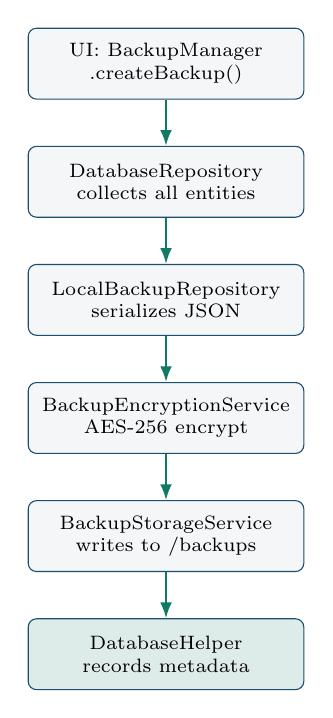
\begin{tikzpicture}[
  node/.style={rectangle, rounded corners=3pt, draw=primaryblue, fill=softgray, minimum width=3.5cm, minimum height=0.9cm, align=center, font=\scriptsize},
  every edge/.style={draw=accentteal, thick, -{Latex[length=2mm]}}
]
\node[node] (ui) at (0,3) {UI: BackupManager\\.createBackup()};
\node[node] (collect) at (0,1.5) {DatabaseRepository\\collects all entities};
\node[node] (serialize) at (0,0) {LocalBackupRepository\\serializes JSON};
\node[node] (encrypt) at (0,-1.5) {BackupEncryptionService\\AES-256 encrypt};
\node[node] (store) at (0,-3) {BackupStorageService\\writes to /backups};
\node[node, fill=accentteal!14] (record) at (0,-4.5) {DatabaseHelper\\records metadata};

\draw (ui) edge (collect);
\draw (collect) edge (serialize);
\draw (serialize) edge (encrypt);
\draw (encrypt) edge (store);
\draw (store) edge (record);
\end{tikzpicture}
\caption{Backup-creation pathway: from user action to encrypted file and metadata record.}
\label{fig:backup-flow}
\end{figure}

\begin{table}[h!]
\centering
\small
\begin{tabular}{p{2.7cm}p{11.5cm}}
\toprule
\textbf{Pathway} & \textbf{Description} \\
\midrule
A. Local write & UI $\to$ \texttt{DatabaseRepository.insertX()} $\to$ \texttt{DatabaseHelper} writes to SQLite. Fully local, no network involvement. \\
B. AI request & UI $\to$ \texttt{AIService} checks consent/cost/policy/quota/connectivity $\to$ if all pass, calls the configured external AI provider $\to$ result returned as a string, quota decremented locally; any failed gate returns a descriptive string instead of throwing. \\
C. Backup creation & See Figure~\ref{fig:backup-flow}. \\
\bottomrule
\end{tabular}
\caption{Summary of the three primary data-flow pathways in the application.}
\end{table}

% ============================================================
%  8. RESULTS & DISCUSSION
% ============================================================
\section{Results and Discussion}
The layered, domain-driven structure kept business logic (scheduling, SM-2, quota gating) concentrated in a small number of testable classes rather than scattered across UI widgets, which is reflected in the unit-test inventory: the three files with the deepest business logic (\texttt{ai\_service\_test.dart}, \texttt{backup\_restore\_test.dart}, \texttt{ai\_service\_retry\_test.dart}) account for over a third of all test lines. The defensive-parsing convention used throughout \texttt{app\_models.dart} proved directly useful in practice, as schema migrations and backup/restore both depend on the same tolerant-parsing contract, and both are exercised by dedicated tests. The consent/quota/connectivity gating pattern in \texttt{AIService} generalizes cleanly: every online feature added to the app (flashcards, quizzes) reuses the same four-check gate rather than reimplementing it, which reduces the surface area for a feature to accidentally bypass user consent.

The principal remaining architectural trade-off is the local database's lack of OS-level encryption, accepted for the current release given the single-user, offline threat model, but flagged explicitly as future hardening work rather than left undocumented.

% ============================================================
%  9. CONCLUSION
% ============================================================
\section{Conclusion and Future Work}
Retainly demonstrates that an offline-first educational tool can still offer adaptive scheduling, spaced repetition, and optional AI assistance without compromising on data locality, user consent, or graceful degradation. The codebase's domain/data/presentation separation, defensive parsing conventions, and consent-gating pattern were validated both by targeted unit tests and by a dedicated security audit that produced four concrete, resolved defects. Future work includes OS-level database encryption (e.g. SQLCipher), server-side-assisted PIN attempt tracking for the (separately tracked) authentication feature, and expanded integration/widget-level test coverage for the planner and revision screens.

\vspace{1cm}
\begin{center}
{\small\itshape --- End of Whitepaper ---}
\end{center}

\end{document}
